\chapter{Software Engineering Process}

As the majority of the work put into this project was in developing the software artifact, I was focused from the beginning on following an effective software engineering process.

\section{Process}
I employed an agile\cite{Agile} methodology throughout my work on this project. 

One of the key Agile principles is to `Deliver working software frequently'\cite{AgileKey}. I planned on fulfilling this from the start, by setting myself intermediary deadlines by which I planned to demo working versions of code. These deadlines were discussed and agreed upon with my supervisor. This allowed me to stay focused on getting the features I needed working, and to avoid premature optimisation.

Another primary principle of the Agile Manifesto is to `Welcome changing requirements, even late in development'\cite{AgileKey}. As an example of this, one of my original requirements involved assessing how accurately my tool could gather people's real world views. After thinking more about the psychological aspects of this question, I decided that it was out of scope, and changed this requirement to a comparatively simple user evaluation. 

\section{Tools}
With this in mind, one of the first tools I employed was Git\cite{Git}.
Considering the length of the project, it was reasonable to suspect that there may come a time when I would have to revert my project to a previous point if something was broken.
Version control software was the obvious solution, and Git is the one I have the most experience with. To complement this, I set up a master GitHub\cite{GitHub} repository to serve as a backup.

In addition to serving as a backup, GitHub provides a good set of project tracking features. 
I considered other tools often used to track projects, such as Trello\cite{Trello}, but in the end decided that GitHub's ability to reference aspects of the code (due to them being stored together) made it better suited for my needs. 
I will outline which features I used here:

\paragraph{Issues} These are the core element of GitHub. Any task that needs completing is documented as an issue.
I kept my issues fairly high-level, as I have found previously that too much detail in issues results in spending excessive amounts of time managing them, and outdated aspects become too common. Figure \ref{fig:issue} shows an example issue.

\begin{figure}[!h]
	\centering
	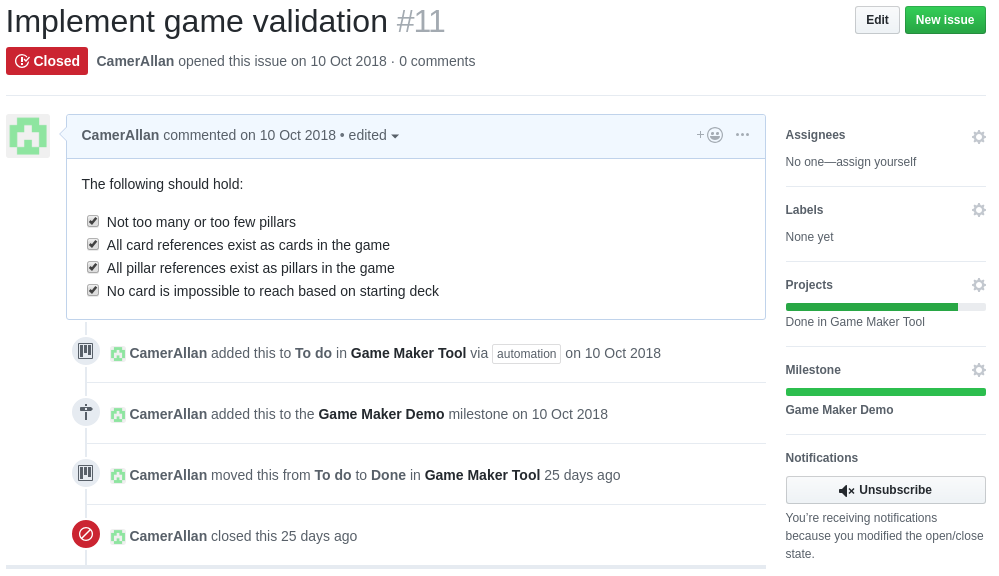
\includegraphics[width=1.0\textwidth]{./images/softeng/issue.png}
	\caption{An example of an issue, note the assigned description, project, and milestone.}
	\label{fig:issue}
\end{figure}

\paragraph{Projects} Issues alone can become unorganised, so I made use of GitHub's projects feature. 
I split my work into four parts - game, game maker, visualisation and backend then made a project for each of these. 
This allowed me to keep issues relating to different parts of the project separate, making it easier to focus on one section at a time.

\begin{figure}[!h]
	\centering
	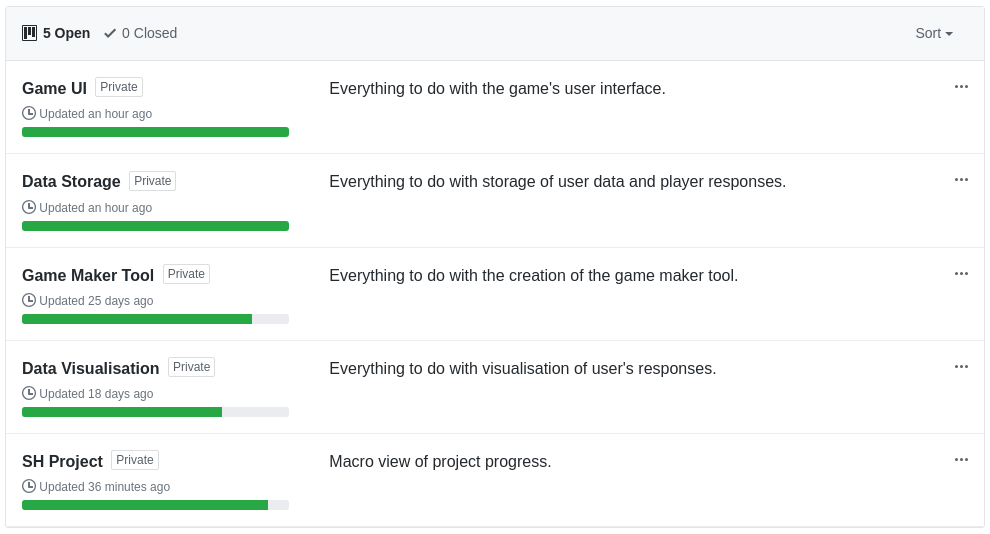
\includegraphics[width=1.0\textwidth]{./images/softeng/projects.png}
	\caption{Project overview page.}
	\label{fig:projects}
\end{figure}

Each project has its own kanban-style board, used to track its progress. 
An example can be seen in figure \ref{fig:board}. Issues assigned to a project start in the \c{todo} column. When being worked on, I would move them into \c{In progress}, and finally when closed they are automatically moved to \c{Done}.

The number of issues in each column defines the project overview, so this can provide a reasonably accurate depiction of the progress of each section.

\begin{figure}[!h]
	\centering
	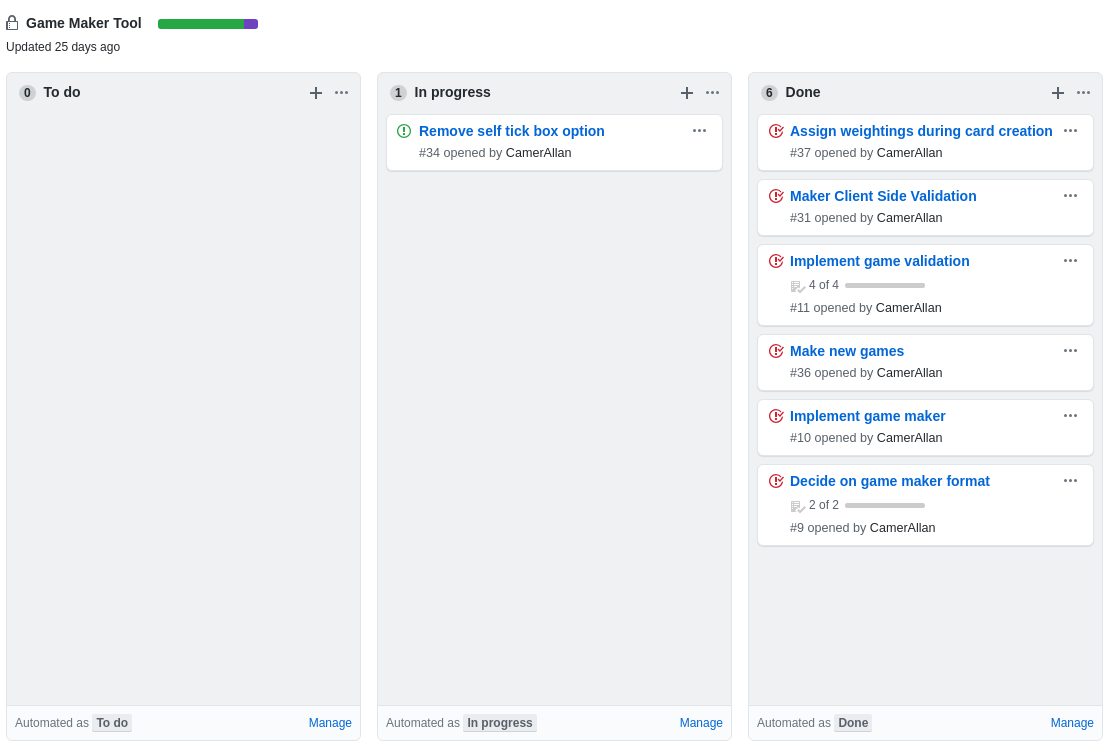
\includegraphics[width=1.0\textwidth]{./images/softeng/board.png}
	\caption{Example project board towards the end of the project.}
	\label{fig:board}
\end{figure}

\paragraph{Milestones} The first step I took in tracking my project was to set my Milestones. These are an aspect of a GitHub project that serve as a deadline, to which issues can be added. 
Completing and closing these issues then automatically provides a visualisation of progress towards a milestone, as can be seen in figures \ref{fig:closed_milestones} and \ref{fig:open_milestones}. 
These made for a helpful overview, which was useful both for myself, and for sharing my progress with my supervisor.

I decided on these milestones early on by estimating the dates by which I could complete core parts of the project. As this was done in advance I was not able to be precise with demo dates, however I completed the vast majority of work for each milestone before the deadline, so I consider this a successful element of my planning.

\begin{figure}[!h]
	\centering
	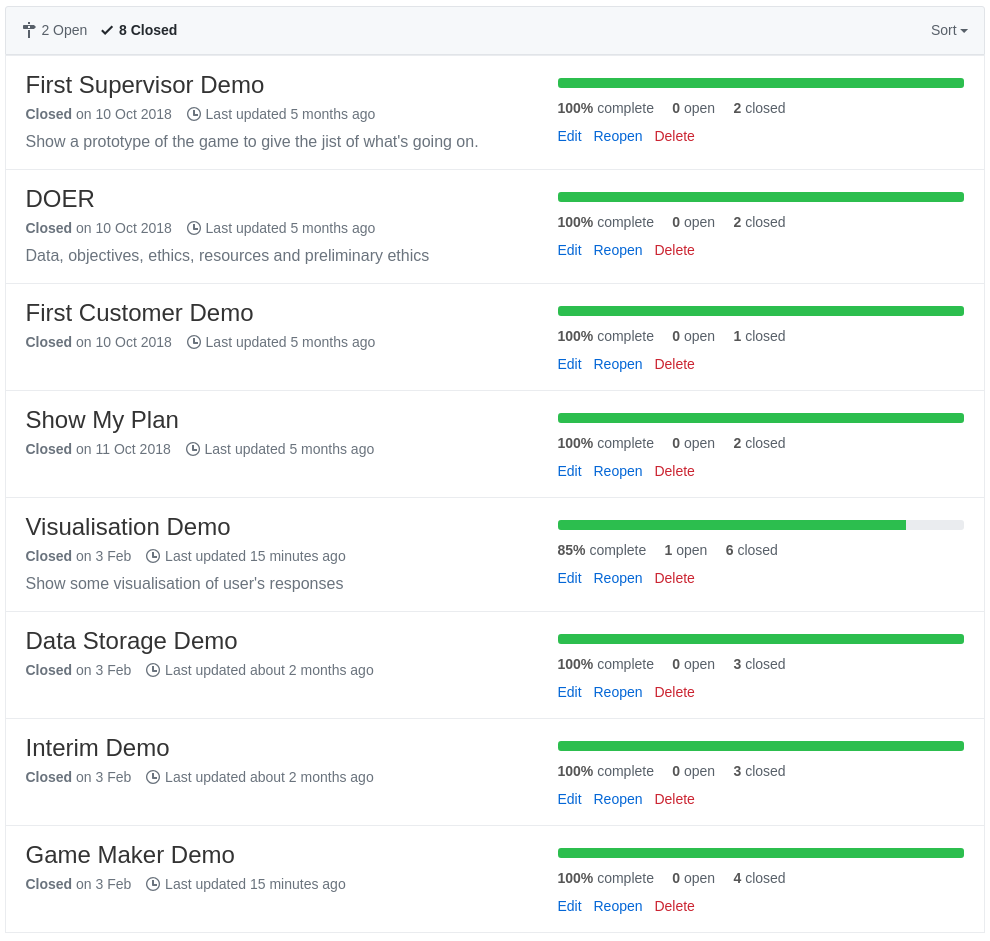
\includegraphics[width=1.0\textwidth]{./images/softeng/closed_milestones.png}
	\caption{Overview of closed (completed) milestones towards the end of the project}
	\label{fig:closed_milestones}
\end{figure}

\begin{figure}[!h]
	\centering
	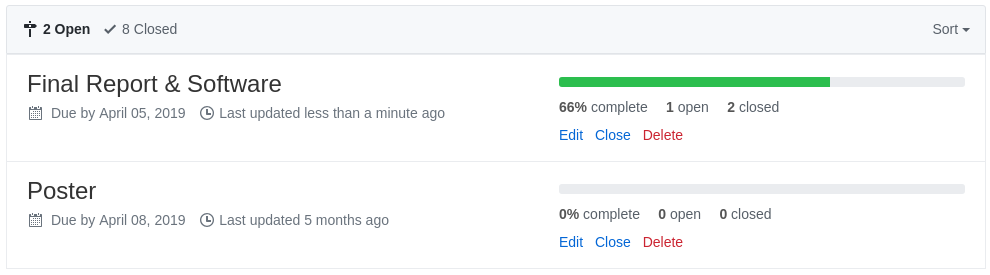
\includegraphics[width=1.0\textwidth]{./images/softeng/open_milestones.png}
	\caption{Overview of open milestones towards the end of the project}
	\label{fig:open_milestones}
\end{figure}

